\documentclass[border=10pt]{standalone}
\usepackage[svgnames]{xcolor}
\usepackage{amsmath}
\usepackage{pgfplots}
\pgfplotsset{compat=newest}
\usepackage[sfdefault]{FiraSans}
\usepackage{FiraMono}
\renewcommand*\familydefault{\sfdefault}
\begin{document}
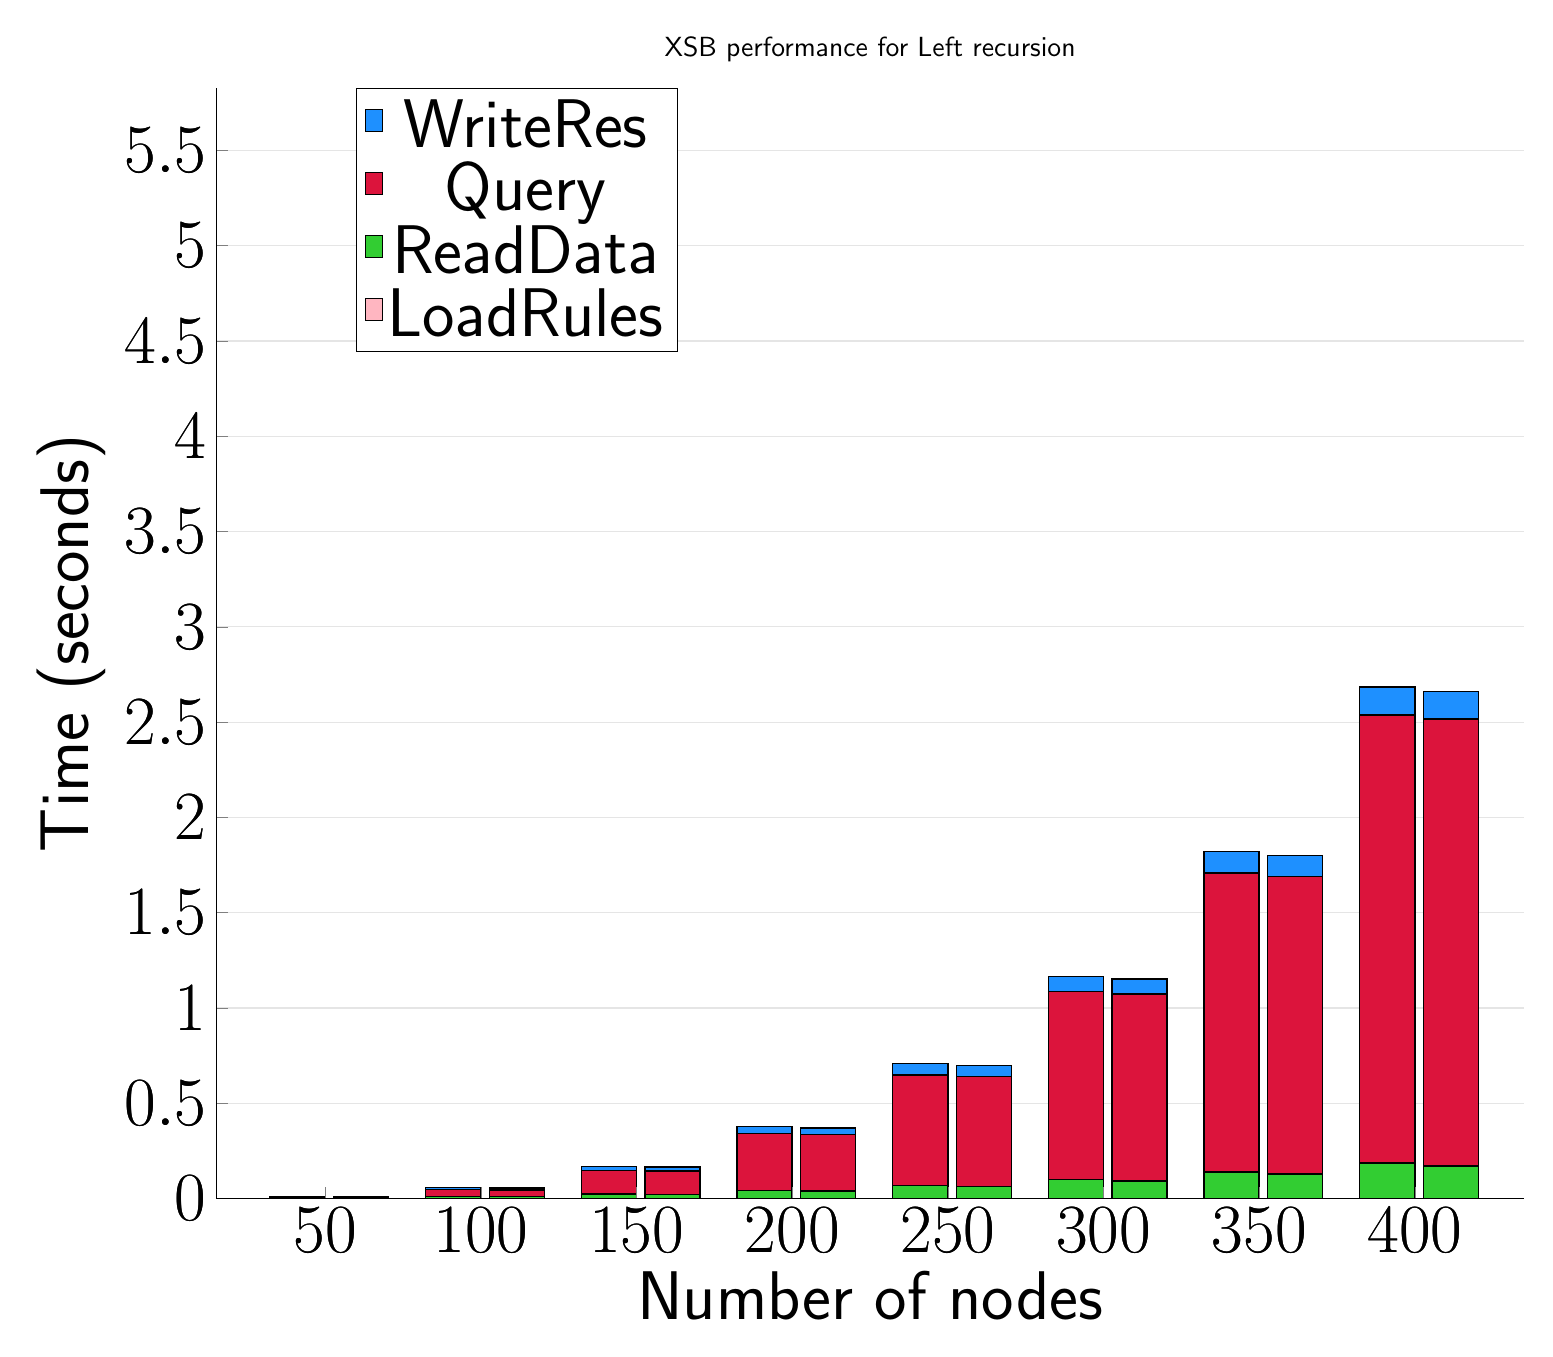
\begin{tikzpicture}
\begin{axis}[
   ybar stacked,
   title={XSB performance for Left recursion},
   bar shift=-10pt,
   width=1.5\textwidth,
   bar width=0.7cm,
   ymajorgrids, tick align=inside,
   major grid style={draw=gray!20},
   xtick=data,
   ymin=0, ymax=5.828503680229188,
   axis x line*=bottom,
   axis y line*=left,
   enlarge x limits=0.1,
   legend style={
       at={(0.23, 1)},
       anchor=north,
       legend columns=1,
       font=\Huge,
   },
   ylabel={Time (seconds)},
   xlabel={Number of nodes},
   label style={font=\Huge},
   tick label style={font=\Huge},
]
\addlegendimage{fill=DodgerBlue, draw=black, line width=0.2pt}
\addlegendentry{WriteRes}
\addlegendimage{fill=Crimson, draw=black, line width=0.2pt}
\addlegendentry{Query}
\addlegendimage{fill=LimeGreen, draw=black, line width=0.2pt}
\addlegendentry{ReadData}
\addlegendimage{fill=LightPink, draw=black, line width=0.2pt}
\addlegendentry{LoadRules}
\addplot +[fill=LightPink, draw=black, line width=0.5pt] coordinates {
    (50, 0.0010782003402709979)
    (100, 0.001044464111328124)
    (150, 0.0010261058807373052)
    (200, 0.0010584592819213878)
    (250, 0.0011057376861572268)
    (300, 0.001086163520812988)
    (350, 0.001104569435119628)
    (400, 0.001141953468322755)
};
\addplot +[fill=LimeGreen, draw=black, line width=0.5pt] coordinates {
    (50, 0.0026242017745971673)
    (100, 0.009995913505554194)
    (150, 0.02300145626068115)
    (200, 0.04218611717224119)
    (250, 0.06739635467529297)
    (300, 0.09910733699798585)
    (350, 0.13866696357727043)
    (400, 0.1845629930496215)
};
\addplot +[fill=Crimson, draw=black, line width=0.5pt] coordinates {
    (50, 0.004538869857788086)
    (100, 0.03598182201385499)
    (150, 0.12323126792907699)
    (200, 0.2980130910873413)
    (250, 0.5808872699737548)
    (300, 0.9856438875198361)
    (350, 1.5685153484344478)
    (400, 2.351499819755552)
};
\addplot +[fill=DodgerBlue, draw=black, line width=0.5pt] coordinates {
    (50, 0.002642726898193359)
    (100, 0.010194325447082509)
    (150, 0.021736359596252704)
    (200, 0.036408805847168005)
    (250, 0.058225822448730515)
    (300, 0.08066709041595393)
    (350, 0.111739373207092)
    (400, 0.14734098911285587)
};
\end{axis}
\begin{axis}[
   ybar stacked,
   bar shift=13pt,
   width=1.5\textwidth,
   bar width=0.7cm,
   ymajorgrids, tick align=inside,
   major grid style={draw=none},
   xtick=data,
   ymin=0, ymax=5.828503680229188,
   axis x line*=none,
   axis y line*=none,
   enlarge x limits=0.1,
   label style={font=\Huge},
   tick label style={font=\Huge},
]
\addplot +[fill=LightPink, draw=black, line width=0.5pt] coordinates {
    (50, 0.0006088999999999997)
    (100, 0.0005952999999999997)
    (150, 0.0005922000000000004)
    (200, 0.0006127999999999998)
    (250, 0.0006257000000000001)
    (300, 0.0006165999999999998)
    (350, 0.0006244999999999998)
    (400, 0.0006453000000000001)
};
\addplot +[fill=LimeGreen, draw=black, line width=0.5pt] coordinates {
    (50, 0.0022530000000000002)
    (100, 0.008904299999999999)
    (150, 0.0207792)
    (200, 0.038480099999999996)
    (250, 0.06126210000000001)
    (300, 0.0909852)
    (350, 0.1278388)
    (400, 0.1712944)
};
\addplot +[fill=Crimson, draw=black, line width=0.5pt] coordinates {
    (50, 0.0045045)
    (100, 0.035778700000000004)
    (150, 0.12264720000000003)
    (200, 0.29655529999999997)
    (250, 0.5789665)
    (300, 0.9814788000000002)
    (350, 1.5632397999999998)
    (400, 2.3444772)
};
\addplot +[fill=DodgerBlue, draw=black, line width=0.5pt] coordinates {
    (50, 0.0023659999999999996)
    (100, 0.009541200000000003)
    (150, 0.020965499999999998)
    (200, 0.03552209999999999)
    (250, 0.056446799999999984)
    (300, 0.07943920000000002)
    (350, 0.10904200000000001)
    (400, 0.1441681)
};
\end{axis}
\end{tikzpicture}

\end{document}
